\documentclass[usenames,dvipsnames]{beamer}
%---- PREAMBLE ----%

% Allows separate files to be used in the main file
\usepackage{subfiles}

% Algorithms
\usepackage{algorithm}
\usepackage[noend]{algpseudocode}
\renewcommand{\algorithmicrequire}{\textbf{Input:}}
\renewcommand{\algorithmicensure}{\textbf{Output:}}
\newcommand{\algorithmicbreak}{\State \textbf{break}}
\newcommand{\Break}{\algorithmicbreak}
\renewcommand{\algorithmicreturn}{\State \textbf{return}}
\newcommand{\algorithmicto}{\textbf{ to }}
\newcommand{\To}{\algorithmicto}
\newcommand{\algorithmicrun}{\State \textbf{call }}
\newcommand{\Run}{\algorithmicrun}
\newcommand{\algorithmicoutput}{\textbf{output }}
\newcommand{\Output}{\algorithmicoutput}
\newcommand{\algorithmictrue}{\textbf{true}}
\newcommand{\True}{\algorithmictrue}
\newcommand{\algorithmicfalse}{\textbf{false}}
\newcommand{\False}{\algorithmicfalse}
\newcommand{\algorithmicand}{\textbf{ and }}
\newcommand{\AAnd}{\algorithmicand}
\newcommand{\algorithmicnot}{\textbf{not}}
\newcommand{\Not}{\algorithmicnot}
\newcommand{\algorithmicor}{\textbf{ or }}
\newcommand{\Or}{\algorithmicor}

% Contains advanced math extensions
\usepackage{amsmath}

% Introduces the *proof* environment and the \theoremstyle command
\usepackage{amsthm}

% Adds new symbols to be used in math mode, e.g. \mathbb
\usepackage{amssymb}

% To declare multiple authors
%\usepackage{authblk}

% Provides extra comands as well as optimisation for producing tables
\usepackage{booktabs}
\newcommand{\ra}[1]{\renewcommand{\arraystretch}{#1}}

% Allows customisation of appearance and placements for figures/tables etc.
\usepackage{caption}

\usepackage{comment}

% Adds support for arbitrarily-deep nested lists
\usepackage[inline]{enumitem}

%Support for changing size of font in table footnotes
%\usepackage{etoolbox}

% Improves the interface for defining floating objects such as figures/tables
\usepackage{float}

%\usepackage{fullpage}

% For easy management of document margins and the document page size
\usepackage[a4paper]{geometry}

% Allows insertion of graphic files within a document
\usepackage{graphicx}

% Manage links within the document or to any URL when you compile in PDF
\usepackage[colorlinks]{hyperref} 
\usepackage[dvipsnames]{xcolor}
%Tikz colours, used in tikz figures only
\colorlet{tBlue}{RoyalBlue!35!Cerulean} %tikz color
\colorlet{tRed}{Red} %tikz color
\definecolor{tGreen}{HTML}{569909} %tikz color
\definecolor{tOrange}{HTML}{FA7602} %tikz color
\definecolor{tLightGreen1}{HTML}{C1E685} %tikz color
\definecolor{tLightOrange1}{HTML}{FFCD4F} %tikz color
\colorlet{tLightGreen}{LimeGreen!70!OliveGreen!45!White}
\colorlet{tLightOrange}{Dandelion!65!White}
\definecolor{tLightPink}{HTML}{FFD4EB} %tikz color
\definecolor{tLightBlue}{HTML}{CEF0FF} %tikz color

%Text colours
\colorlet{myRed}{Red!50!OrangeRed}
\definecolor{myOrange}{HTML}{FA7602}
\definecolor{myGreen}{HTML}{569909}
\definecolor{myAqua}{HTML}{00B1BA} %02BEB8
\definecolor{myBlue}{HTML}{0095FF} %00B3FF
\colorlet{myPurple}{Orchid} 
\colorlet{myPink}{Rhodamine!65!Lavender}
\colorlet{myGray}{Gray!90!White}

\hypersetup{
		linkcolor=myPurple,
		citecolor=myAqua,
		urlcolor=black
}

% The document class `elsarticle` uses the \AtBeginDocument comman to define the colour of all link types as blue, so we use the \AtBeginDocument command again to overwrite the colour settings to the colors we choose. REMEMBER TO REMOVE THIS BEFORE SUBMITTING.
%\AtBeginDocument{% 
%	\hypersetup{
%		linkcolor=myPurple,
%		citecolor=myAqua,
%		urlcolor=black
%	}
%} %end of \AtBeginDocument

\newcommand{\intro}[1]{{\color{myOrange}#1}} % \intro{<text>}, makes <text> orange, use to highlight things to do, urgent, or revisit in introduction section

\newcommand{\ahc}[1]{{\color{myBlue}#1}} % \ahc{<text>}, makes <text> blue, use to highlight things to do, urgent, or revisit in AHC section

\newcommand{\heur}[1]{{\color{myPink}#1}} % \scspp{<text>}, makes <text> pink, use to highlight things to do, urgent, or revisit in SCSPP section

\newcommand{\ea}[1]{{\color{myRed}#1}} % \ea{<text>}, makes <text> red, use to highlight things to do, urgent, or revisit in EA section

\newcommand{\cmsa}[1]{{\color{myGreen}#1}} % \cmsa{<text>}, makes <text> green, use to highlight things to do, urgent, or revisit in CMSA section

\newcommand{\conc}[1]{{\color{myPurple}#1}} % \conc{<text>}, makes <text> purple, use to highlight things to do, urgent, or revisit in Conclusion section

\newcommand{\note}[1]{{\color{myPurple}#1}} % \note{<text>}, makes <text> turquoise, use to highlight things to do, urgent, or revisit in any section


\newcommand{\alert}[1]{{\color{myRed}#1}} % \alert{<text>}, makes <text> red, use to highlight things to do, urgent, or revisit.

\newcommand{\done}[1]{{\color{myGray}#1}} % \done{<text>}, makes <text> gray, use to highlight things that are not required or should be ignored.

\newcommand{\ialert}[1]{{\color{myRed}\item#1}} % \ialert{<text>}, makes <text> a red bullet point, use for bullet points of things to do, urgent, or revisit.

\newcommand{\idone}[1]{{\color{myGray}\item#1}} % \idone{<text>}, makes <text> a gray bullet point, use for bullet points that have been completed, that are not required or should be ignored.

\renewcommand{\idone}[1]{} % hides all \idone bullet points

% Successor of amsmath
\usepackage{mathtools}

\usepackage{multirow}

% No indentation, space between paragraphs
%\usepackage{parskip}

\usepackage[round]{natbib}

%Include standalone .tex files
\usepackage{standalone}

% Define multiple floats (figures/tables) within one environment with individual captions 1a, 1b etc
\usepackage{subcaption}

%\usepackage[caption=false,font=footnotesize]{subfig}

\usepackage{tabularx}

\usepackage{threeparttable}
%\appto\TPTnoteSettings{\footnotesize} % Change font size of table footnotes to footnotesize

\usepackage{tikz}
\usetikzlibrary{shapes.geometric}

\usepackage{wrapfig}

% Need \usepackage{mathtools} to use floor/ceil below.
% Example: \floor*{\frac{x}{2}}, \ceil*{\frac{x}{2}}
% The asterisk resizes floor/ceil brackets.
\DeclarePairedDelimiter{\floor}{\lfloor}{\rfloor}
\DeclarePairedDelimiter{\ceil}{\lceil}{\rceil}

%Theorem style
%\theoremstyle{plain}% default
\newtheorem{theorem}{Theorem}
%\newtheorem{corollary}{Corollary}
\newtheorem{definition}{Definition}

%\theoremstyle{definition}
%\newtheorem{definition}{Definition}
%\newtheorem{proposition}{Proposition}
%\newtheorem{exmp}{Example}[section]
\setbeamertemplate{caption}{\raggedright\insertcaption\par}

\begin{document}

\title{Increasing Productivity in the Domiciliary Care Sector Through Automated Routing and Scheduling of Carers}
\date{}
\author{A. L. Hawa, C. Lamas-Fernandez, A. Martinez-Sykora, C. Currie, T. Monks, T. Chalklen}
\titlegraphic{
\includegraphics[height=1.2cm]{figures/sotonabicare2.png}}
\maketitle

%\section{Introduction}

\begin{frame}{Task}
To create an efficient route and schedule for each carer such that all patients (jobs) are visited at the correct times by suitable carers.
\small
\begin{multicols}{2}
	\begin{itemize}
		\item Assign jobs to sufficiently skilled carer(s)
		\item Assign jobs to preferred carers(s)
		\item Assign carers to preferred jobs
		\item Workload balance %($\overline{B}$)
		\item Minimise waiting times %($\overline{W}$)
		\item Minimise tardiness %($\overline{Z}$)
		\item Minimise overtime %($\overline{O}$)
		\item Minimise travel time %($\overline{T}$)
		\item Minimise travel distance*
		%\item Assign jobs and carers according to preferences ($\overline{P}$)
	\end{itemize}	
\end{multicols}	
\end{frame}	

\begin{frame}{Current Model and Approach}
%\begin{multicols}{2}
	\begin{itemize}
		\item Weighted objective function 
		\item Produce multiple schedules depending on the desired objective
		\item Currently implemented in C++ and Python
	\end{itemize}	
%\end{multicols}	
\end{frame}

\begin{frame}{Data}
This is required from each location:
\footnotesize
\begin{multicols}{2}
	\begin{itemize}
		\item Total number of patients/carers in each location
		\item Max travel distance (route/radius)
		\item Skills of carers
		\item Time window of each job
		\item Patient preferences: language, gender of carers, personal
		\item Carer preferences: gender of patient, allergies, personal
		\item Length of day for carers (full/half/flexible)
		\item Number of DS/synchronised services
		\item Distinct job types?
		\item Carers ``on call''
		\item Strength of preferences
	\end{itemize}	
\end{multicols}	
\end{frame}

\begin{frame}{Queries}
\scriptsize
%\begin{multicols}{2}
	\begin{itemize}
		\item \note{Desired objective(s)}
		\item Are there skill ``levels'' for carers?
		\item Distinct job types or customised per job
		\item Jobs that \emph{cannot} start late
		\item Lunch breaks
		\item Parking availability at patient's home
		\item PPE/COVID-19 conditions
		\item Frequency of schedule formation
		\item Database/software currently used
		\item Hard and soft constraints
		\item Any additional constraints?
		\item Who will be using the application?
		\item Additional carers available?
	\end{itemize}	
%\end{multicols}
\end{frame}


\begin{frame}{Rerouting and Rescheduling (R\&R)}
In the event of an unexpected disruption, the original plan may need to be updated to accommodate any changes that occur.

\note{Which of these do we need to address?}
\small
\begin{itemize}
	\item Cancellation of a service
	\item Addition of a new service (single or double)
	\item Modification of a service (single or double)
	\item Patient emergency, carer remains with patient
	\item Increase in skill level of service
	\item Increase in number of carers required for a service
	\item Carer unwell at beginning/during the day or personal emergency
	\item Carer requiring urgent assistance from another carer
\end{itemize}	
\end{frame}

\begin{frame}{Meeting}
\small
\begin{itemize}
	\item EasyLog only has details of time/length of job
	\item Preferences/carer skills/client needs are known by staff only
	\item No jobs between 2-4pm
	\item Day in two shifts: 7am-2pm, 4pm-10pm
	\item ``Ideal rotas'' on EasyLog
	\item Availability of extra carers (e.g. part-time, can help with issues)
	\item TW 15mins before and after start time
	\item QR code carer clock in/out, not accurate
	\item Larger gaps between jobs for new carers, e.g. +10mins travel time
	\item Continuity of care
\end{itemize}	
	
\end{frame}

\begin{frame}{Literature}

\end{frame}

\begin{frame}{Comparison}
\small
\begin{multicols}{3}	
\begin{block}{Hampshire}
	\begin{itemize}
		\item Carers = 15
		\item Clients = 34
		\item Jobs = 480
	\end{itemize}
\end{block}
\begin{block}{Monmouth}
	\begin{itemize}
		\item Carers = 23
		\item Clients = 47
		\item Jobs = 735
	\end{itemize}
\end{block}
\begin{block}{Aldershot}
	\begin{itemize}
		\item Carers = 9
		\item Clients = 19
		\item Jobs = 184
	\end{itemize}
\end{block}
\end{multicols}	
\end{frame}

\begin{frame}{Comparison: Hampshire Time and Distance}
	\begin{figure}
		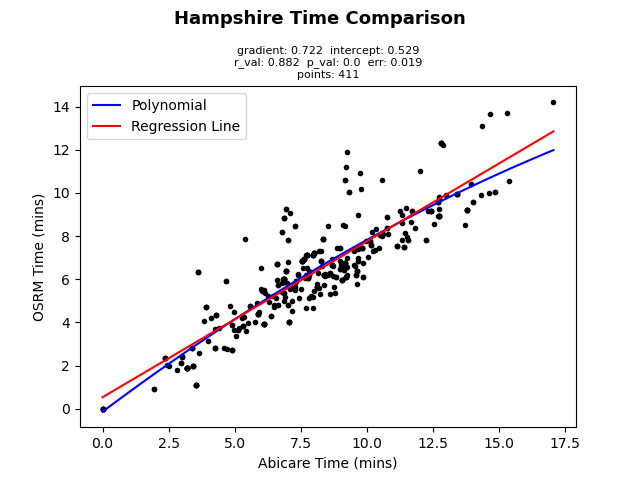
\includegraphics[width=0.5\linewidth]{figures/Hampshire_time_comparison_abi}%
		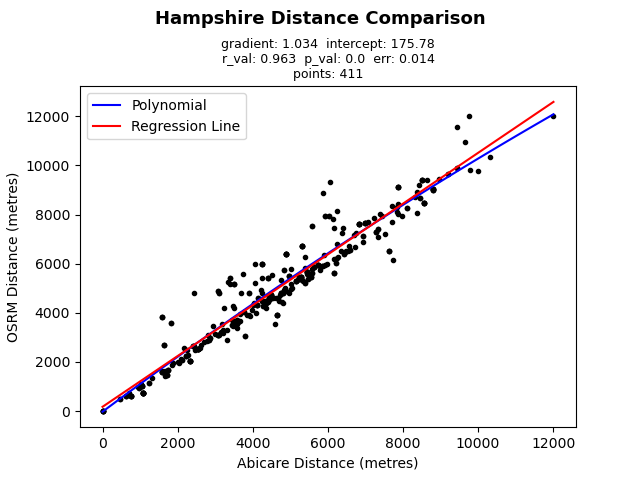
\includegraphics[width=0.5\linewidth]{figures/Hampshire_dist_comparison_abi}
	\end{figure}
\end{frame}

\begin{frame}{Comparison: Monmouth Time and Distance}
	\begin{figure}
		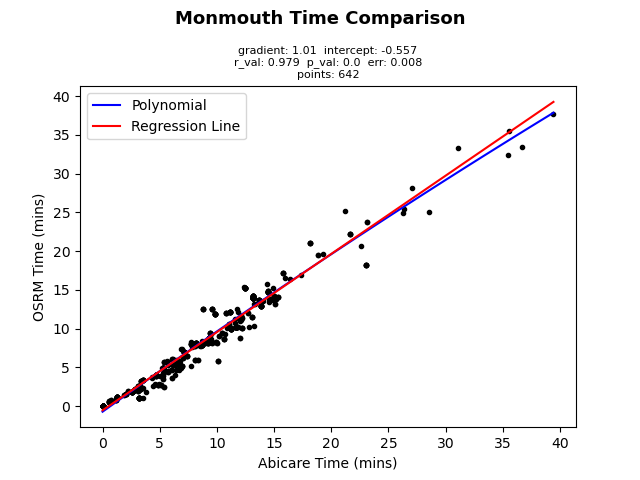
\includegraphics[width=0.5\linewidth]{figures/Monmouth_time_comparison_abi}%
		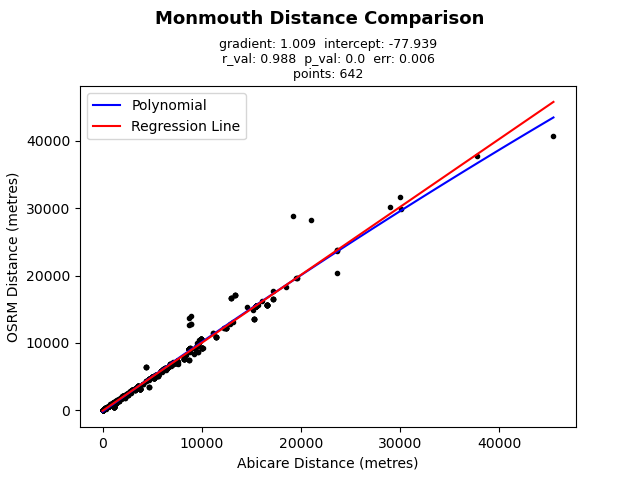
\includegraphics[width=0.5\linewidth]{figures/Monmouth_dist_comparison_abi}
	\end{figure}
\end{frame}

\begin{frame}{Comparison: Aldershot Time and Distance}
	\begin{figure}
		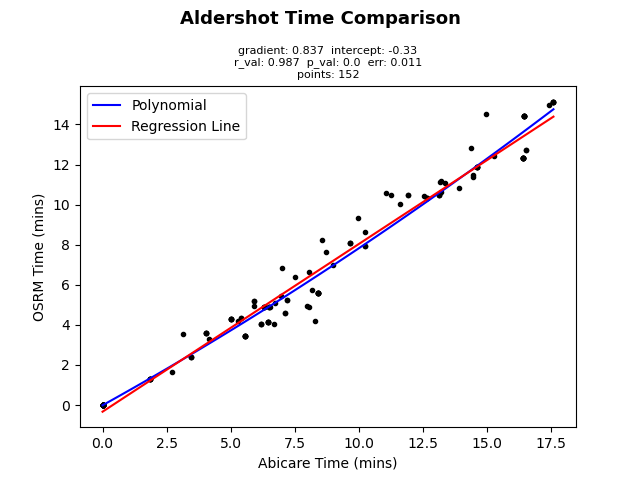
\includegraphics[width=0.5\linewidth]{figures/Aldershot_time_comparison_abi}%
		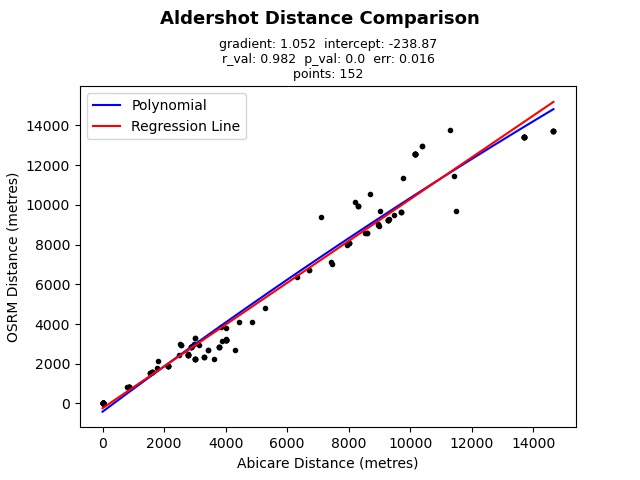
\includegraphics[width=0.5\linewidth]{figures/Aldershot_dist_comparison_abi}
	\end{figure}
\end{frame}

\begin{frame}{Comparison: Hampshire Peak/Off-Peak Times}
	\begin{figure}
		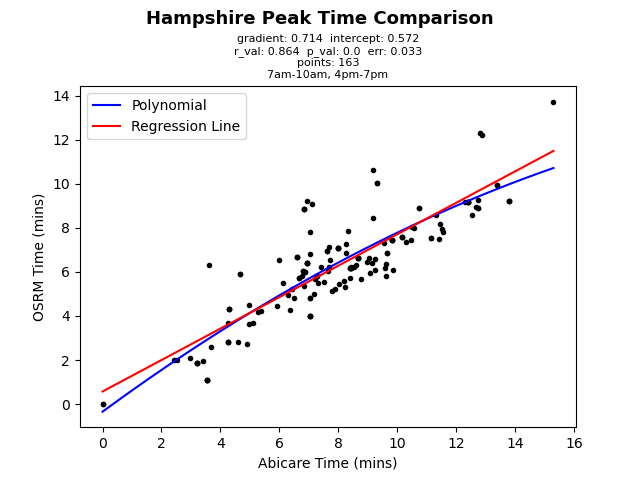
\includegraphics[width=0.5\linewidth]{figures/Hampshire_peaktime_comparison_abi}%
		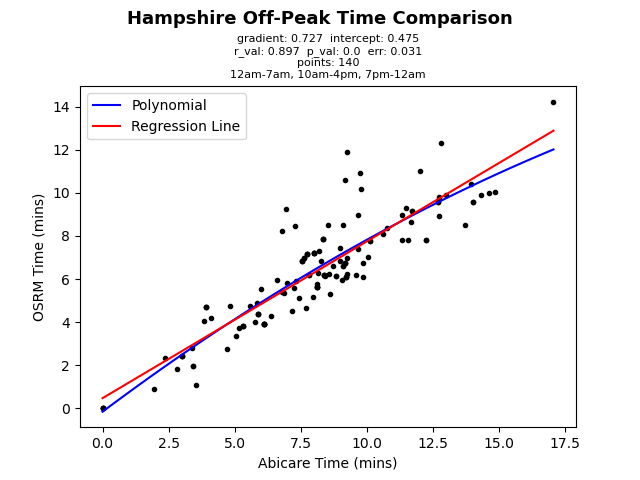
\includegraphics[width=0.5\linewidth]{figures/Hampshire_offpeaktime_comparison_abi}
	\end{figure}
\end{frame}

\begin{frame}{Comparison: Monmouth Peak/Off-Peak Times}
	\begin{figure}
		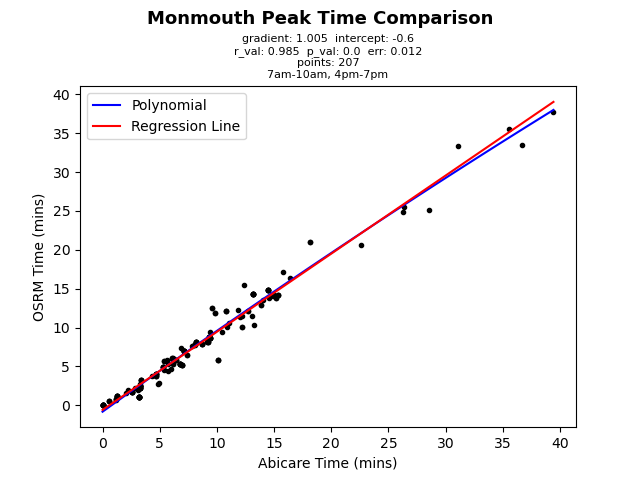
\includegraphics[width=0.5\linewidth]{figures/Monmouth_peaktime_comparison_abi}%
		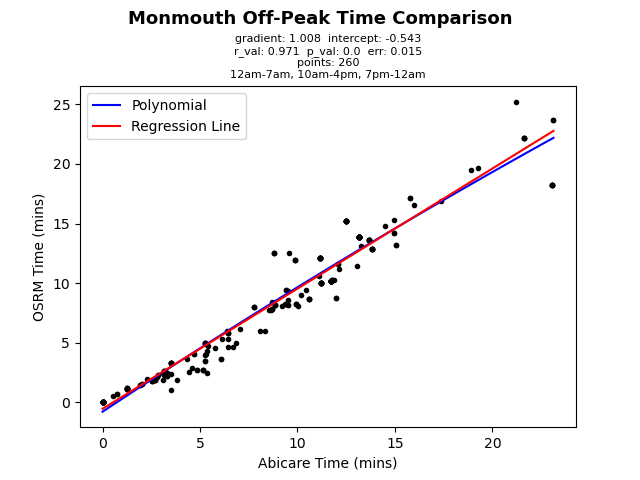
\includegraphics[width=0.5\linewidth]{figures/Monmouth_offpeaktime_comparison_abi}
	\end{figure}
\end{frame}

\begin{frame}{Comparison: Aldershot Peak/Off-Peak Times}
	\begin{figure}
		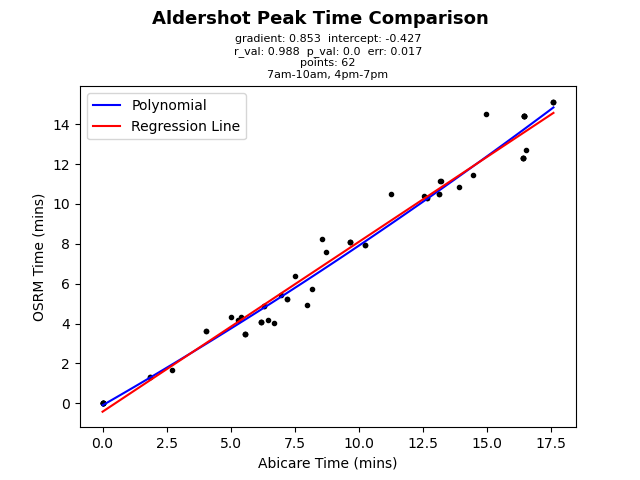
\includegraphics[width=0.5\linewidth]{figures/Aldershot_peaktime_comparison_abi}%
		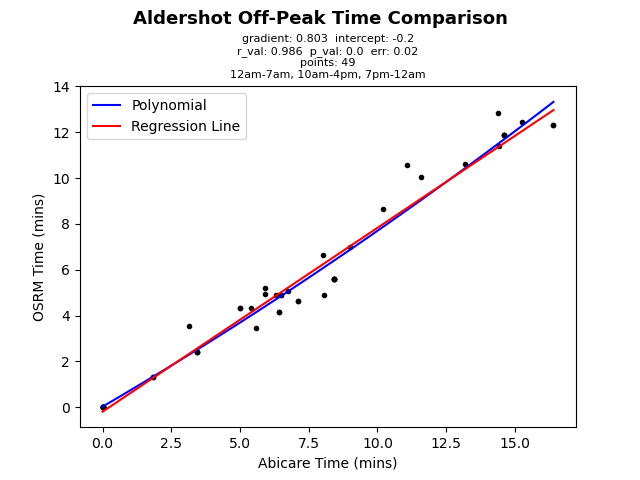
\includegraphics[width=0.5\linewidth]{figures/Aldershot_offpeaktime_comparison_abi}
	\end{figure}
\end{frame}

\begin{frame}
	\begin{figure}
		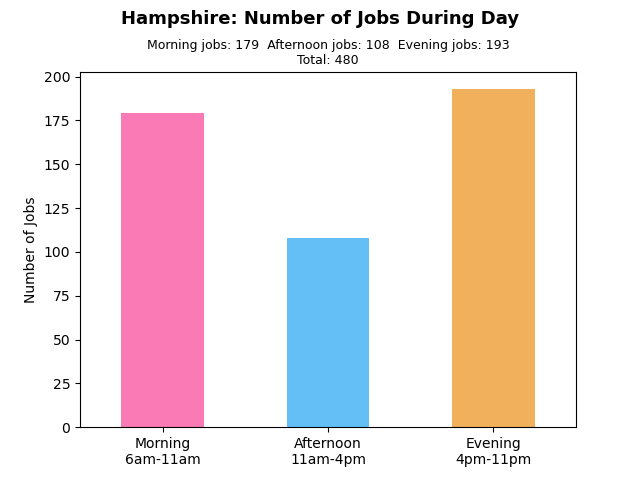
\includegraphics[width=0.5\textwidth]{figures/Hampshire_timeofday_jobs_abi}
	\end{figure}
	\vspace*{-0.9cm}
	\begin{columns}[T]
		\begin{column}{0.5\textwidth}
			\begin{figure}
				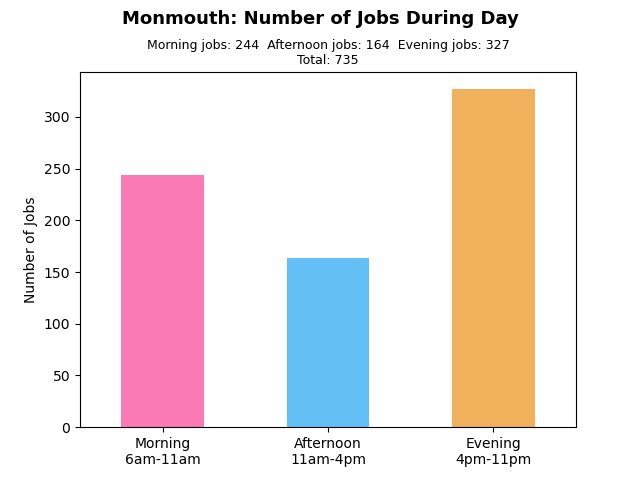
\includegraphics[width=\textwidth]{figures/Monmouth_timeofday_jobs_abi}
			\end{figure}
		\end{column}%
		\begin{column}{0.5\textwidth}
			\begin{figure}
				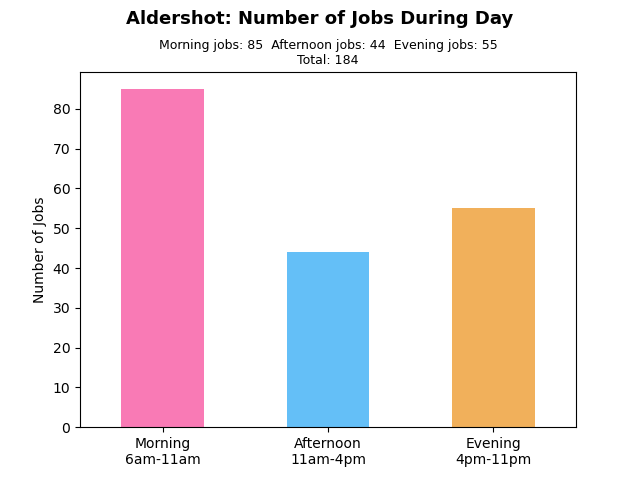
\includegraphics[width=\textwidth]{figures/Aldershot_timeofday_jobs_abi}
			\end{figure}
		\end{column}
	\end{columns}
\end{frame}

\begin{frame}
	\begin{figure}
		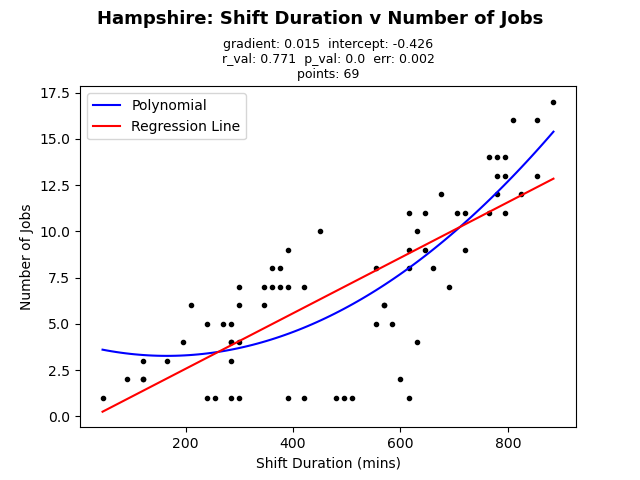
\includegraphics[width=0.5\textwidth]{figures/Hampshire_shift_jobs_abi}
	\end{figure}
	\vspace*{-0.8cm}
	\begin{columns}[T]
		\begin{column}{0.5\textwidth}
			\begin{figure}
				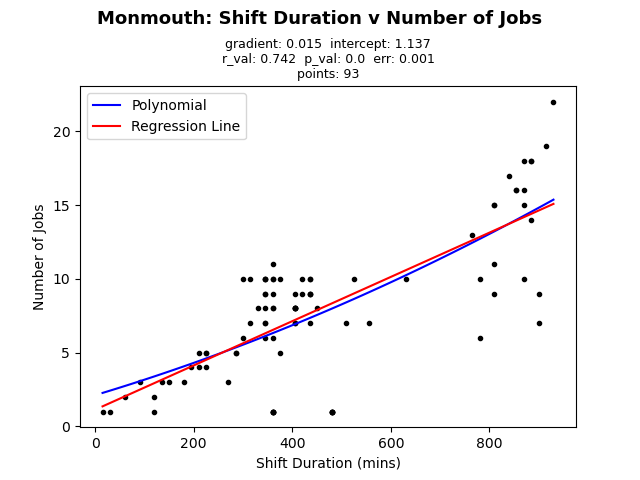
\includegraphics[width=\textwidth]{figures/Monmouth_shift_jobs_abi}
			\end{figure}
		\end{column}%
		\begin{column}{0.5\textwidth}
			\begin{figure}
				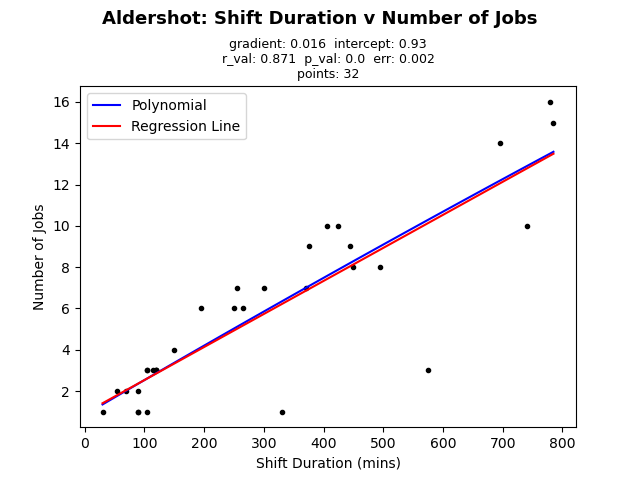
\includegraphics[width=\textwidth]{figures/Aldershot_shift_jobs_abi}
			\end{figure}
		\end{column}
	\end{columns}
\end{frame}



\begin{frame}{Comparison: Total Time (minutes)}
\scriptsize
\begin{table}
%\caption{Comparison}
\renewcommand{\arraystretch}{1.5}
\begin{tabular}{ccrrcrrcrr}\toprule
	&& \multicolumn{2}{c}{Hampshire} && \multicolumn{2}{c}{Monmouth} && \multicolumn{2}{c}{Aldershot} \\
	\cmidrule{3-4} \cmidrule{6-7} \cmidrule{9-10}
	\multicolumn{1}{c}{Date} && \multicolumn{1}{c}{Abicare} & \multicolumn{1}{c}{DST} && \multicolumn{1}{c}{Abicare} & \multicolumn{1}{c}{DST} && \multicolumn{1}{c}{Abicare} & \multicolumn{1}{c}{DST} \\
	\midrule
	02-Nov && 5640.00 & \gre{5452.46} && 6285.00 & \gre{5851.16} && 1480.00 & \gre{1449.90}\\
	03-Nov && 5460.00 & \gre{5282.68} && 6030.00 & \gre{5758.70} && 1080.00 & \gre{1015.74}\\
	04-Nov && 5160.00 & \gre{4996.38} && 6135.00 & \gre{6044.82} && 1355.00 & \gre{1321.32}\\
	05-Nov && 5265.00 & \gre{5089.72} && 7200.00 & \gre{6955.46} && 2000.00 & \gre{1905.00}\\
	06-Nov && 4875.00 & \gre{4617.36} && 7455.00 & \gre{7100.96} && 1470.00 & \gre{1345.28}\\
	07-Nov && 3780.00 & \gre{3616.35} && 4845.00 & \gre{4574.79} && 1065.00 & \gre{1005.92}\\
	08-Nov && 3720.00 & \gre{3608.01} && 4470.00 & \gre{4380.78} && 1050.00 & \gre{1006.87}\\
	\bottomrule
\end{tabular}
\end{table}%
\end{frame}

\begin{frame}{Comparison: Total Travel Time (minutes)}
\scriptsize
\begin{table}
%\caption{Comparison}
\renewcommand{\arraystretch}{1.5}
\begin{tabular}{ccrrcrrcrr}\toprule
	&& \multicolumn{2}{c}{Hampshire} && \multicolumn{2}{c}{Monmouth} && \multicolumn{2}{c}{Aldershot} \\
	\cmidrule{3-4} \cmidrule{6-7} \cmidrule{9-10}
	\multicolumn{1}{c}{Date} && \multicolumn{1}{c}{Abicare} & \multicolumn{1}{c}{DST} && \multicolumn{1}{c}{Abicare} & \multicolumn{1}{c}{DST} && \multicolumn{1}{c}{Abicare} & \multicolumn{1}{c}{DST} \\
	\midrule
	02-Nov && 475.00 & \gre{232.28} && 722.55 & \gre{687.00} && 192.77 & \gre{124.81}\\
	03-Nov && 489.88 & \gre{227.02} && \red{728.62} & 745.88 && 166.05 & \gre{119.21}\\
	04-Nov && 490.77 & \gre{242.58} && \red{769.78} & 895.18 && 178.28 & \gre{119.79}\\
	05-Nov && 490.42 & \gre{271.44} && 798.20 & \gre{687.87} && 211.58 & \gre{122.75}\\
	06-Nov && 479.50 & \gre{243.76} && \red{864.52} & 920.79 && 152.97 & \gre{108.11}\\
	07-Nov && 452.67 & \gre{243.81} && \red{694.07} & 779.27 && 167.70 & \gre{108.08}\\
	08-Nov && 405.41 & \gre{223.68} && \red{666.17} & 802.96 && 176.48 & \gre{119.98}\\
	\bottomrule
\end{tabular}
\end{table}%
\end{frame}

\begin{frame}{Comparison NEW: Total Travel Time (minutes)}
	\scriptsize
	\begin{table}
		%\caption{Comparison}
		\renewcommand{\arraystretch}{1.5}
		\begin{tabular}{ccrrcrrcrr}\toprule
			&& \multicolumn{2}{c}{Hampshire} && \multicolumn{2}{c}{Monmouth} && \multicolumn{2}{c}{Aldershot} \\
			\cmidrule{3-4} \cmidrule{6-7} \cmidrule{9-10}
			\multicolumn{1}{c}{Date} && \multicolumn{1}{c}{Abicare} & \multicolumn{1}{c}{DST} && \multicolumn{1}{c}{Abicare} & \multicolumn{1}{c}{DST} && \multicolumn{1}{c}{Abicare} & \multicolumn{1}{c}{DST} \\
			\midrule
			02-Nov && 372.88 & \gre{232.28} && \red{674.46} & 687.00 && 153.05 & \gre{124.81}\\
			03-Nov && 381.58 & \gre{227.02} && \red{675.89} & 745.88 && 129.47 & \gre{119.21}\\
			04-Nov && 384.52 & \gre{242.58} && \red{722.42} & 895.18 && 141.19 & \gre{119.79}\\
			05-Nov && 389.95 & \gre{271.44} && 745.86 & \gre{687.87} && 168.99 & \gre{122.7}5\\
			06-Nov && 378.22 & \gre{243.76} && \red{824.72} & 920.79 && 123.08 & \gre{108.11}\\
			07-Nov && 356.83 & \gre{243.81} && \red{661.50} & 779.27 && 133.91 & \gre{108.08}\\
			08-Nov && 324.72 & \gre{223.68} && \red{636.07} & 802.96 && 142.60 & \gre{119.98}\\
			\bottomrule
		\end{tabular}
	\end{table}%
\end{frame}

\begin{frame}{Comparison: Total Waiting Time (minutes)}
\scriptsize
\begin{table}
%\caption{Comparison}
\renewcommand{\arraystretch}{1.5}
\begin{tabular}{ccrrcrrcrr}\toprule
	&& \multicolumn{2}{c}{Hampshire} && \multicolumn{2}{c}{Monmouth} && \multicolumn{2}{c}{Aldershot} \\
	\cmidrule{3-4} \cmidrule{6-7} \cmidrule{9-10}
	\multicolumn{1}{c}{Date} && \multicolumn{1}{c}{Abicare} & \multicolumn{1}{c}{DST} && \multicolumn{1}{c}{Abicare} & \multicolumn{1}{c}{DST} && \multicolumn{1}{c}{Abicare} & \multicolumn{1}{c}{DST} \\
	\midrule
	02-Nov && \red{1595.00} & 1650.18 && 1407.45 & \gre{1009.16} && \red{222.23} & 260.09\\
	03-Nov && \red{1580.12} & 1665.65 && 1026.38 & \gre{737.81} && 73.95 & \gre{56.53}\\
	04-Nov && \red{1189.23} & 1273.80 && 775.22 & \gre{559.64} && \red{36.72} & 61.53\\
	05-Nov && \red{1159.58} & 1203.28 && 1661.80 & \gre{1527.59} && 338.42 & \gre{332.25}\\
	06-Nov && 1065.50 & \gre{1043.60} && 1505.48 & \gre{1095.16} && 402.03 & \gre{322.17}\\
	07-Nov && \red{957.33} & 1002.54 && 790.93 & \gre{435.51} && \red{212.30} & 212.84\\
	08-Nov && \red{1019.59} & 1089.32 && 548.83 & \gre{322.82} && \red{143.52} & 156.89\\
	\bottomrule
\end{tabular}
\end{table}%
\end{frame}

\begin{frame}{Comparison NEW: Total Waiting Time (minutes)}
	\scriptsize
	\begin{table}
		%\caption{Comparison}
		\renewcommand{\arraystretch}{1.5}
		\begin{tabular}{ccrrcrrcrr}\toprule
			&& \multicolumn{2}{c}{Hampshire} && \multicolumn{2}{c}{Monmouth} && \multicolumn{2}{c}{Aldershot} \\
			\cmidrule{3-4} \cmidrule{6-7} \cmidrule{9-10}
			\multicolumn{1}{c}{Date} && \multicolumn{1}{c}{Abicare} & \multicolumn{1}{c}{DST} && \multicolumn{1}{c}{Abicare} & \multicolumn{1}{c}{DST} && \multicolumn{1}{c}{Abicare} & \multicolumn{1}{c}{DST} \\
			\midrule
			02-Nov && 1697.12 & \gre{1650.18} && 1455.54 & \gre{1009.16} && 261.95 & \gre{260.09}\\
			03-Nov && 1688.42 & \gre{1665.65} && 1079.11 & \gre{737.81} && 110.53 & \gre{56.53}\\
			04-Nov && 1295.48 & \gre{1273.80} && 822.58 & \gre{559.64} && 73.81 & \gre{61.53}\\
			05-Nov && 1260.05 & \gre{1203.28} && 1714.14 & \gre{1527.59} && 381.01 & \gre{332.25}\\
			06-Nov && 1166.78 & \gre{1043.60} && 1545.28 & \gre{1095.16} && 431.92 & \gre{322.17}\\
			07-Nov && 1053.17 & \gre{1002.54} && 823.50 & \gre{435.51} && 246.09 & \gre{212.84}\\
			08-Nov && 1100.28 & \gre{1089.32} && 578.93 & \gre{322.82} && 177.41 & \gre{156.89}\\
			\bottomrule
		\end{tabular}
	\end{table}%
\end{frame}

\begin{frame}{Comparison: Total Travel Distance (km)}
	\scriptsize
	\begin{table}
		%\caption{Comparison}
		\renewcommand{\arraystretch}{1.5}
		\begin{tabular}{ccrrcrrcrr}\toprule
			&& \multicolumn{2}{c}{Hampshire} && \multicolumn{2}{c}{Monmouth} && \multicolumn{2}{c}{Aldershot} \\
			\cmidrule{3-4} \cmidrule{6-7} \cmidrule{9-10}
			\multicolumn{1}{c}{Date} && \multicolumn{1}{c}{Abicare} & \multicolumn{1}{c}{DST} && \multicolumn{1}{c}{Abicare} & \multicolumn{1}{c}{DST} && \multicolumn{1}{c}{Abicare} & \multicolumn{1}{c}{DST} \\
			\midrule
			02-Nov && 288.26 & \gre{161.16} && \red{497.03} & 569.09 && 127.14 & \gre{100.00}\\
			03-Nov && 307.63 & \gre{153.31} && \red{502.23} & 662.55 && 106.41 & \gre{99.03}\\
			04-Nov && 301.65 & \gre{165.69} && \red{550.60} & 822.70 && 108.11 & \gre{90.21}\\
			05-Nov && 302.08 & \gre{193.55} && \red{561.90} & 578.20 && 129.57 & \gre{92.00}\\
			06-Nov && 301.39 & \gre{167.34} && \red{639.99} & 831.14 && 98.11 & \gre{83.70}\\
			07-Nov && 291.58 & \gre{176.95} && \red{503.89} & 662.54 && 110.56 & \gre{82.77}\\
			08-Nov && 250.77 & \gre{160.10} && \red{489.51} & 676.26 && 113.47 & \gre{91.53}\\
			\bottomrule
		\end{tabular}
	\end{table}%
\end{frame}

\begin{comment}
\begin{frame}{Comparison}
	\begin{figure}[T]
		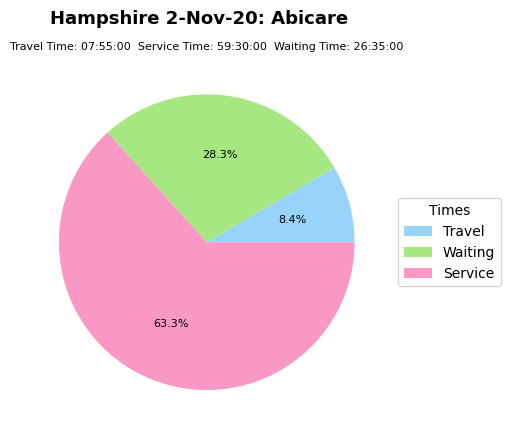
\includegraphics[width=0.5\linewidth]{figures/2_Nov_20_Hampshire_time_info_abi}%
		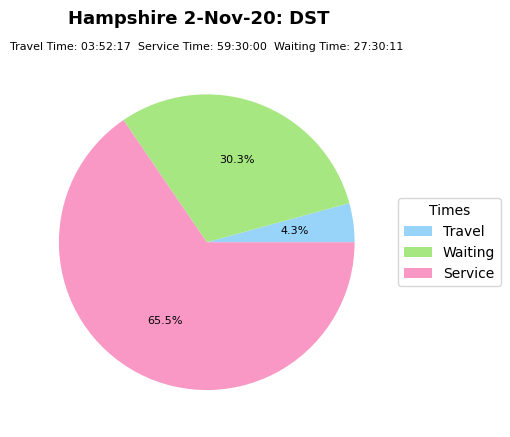
\includegraphics[width=0.5\linewidth]{figures/2_Nov_20_Hampshire_time_info_dst}
	\end{figure}
\end{frame}

\begin{frame}{Comparison}
	\begin{figure}[T]
		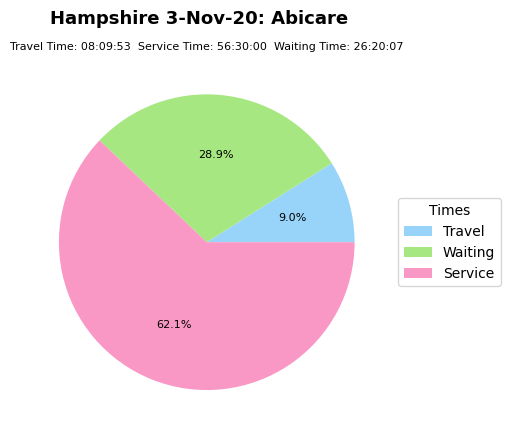
\includegraphics[width=0.5\linewidth]{figures/3_Nov_20_Hampshire_time_info_abi}%
		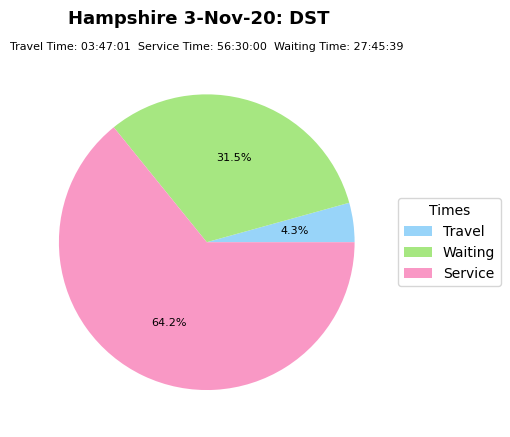
\includegraphics[width=0.5\linewidth]{figures/3_Nov_20_Hampshire_time_info_dst}
	\end{figure}
\end{frame}

\begin{frame}{Comparison}
	\begin{figure}[T]
		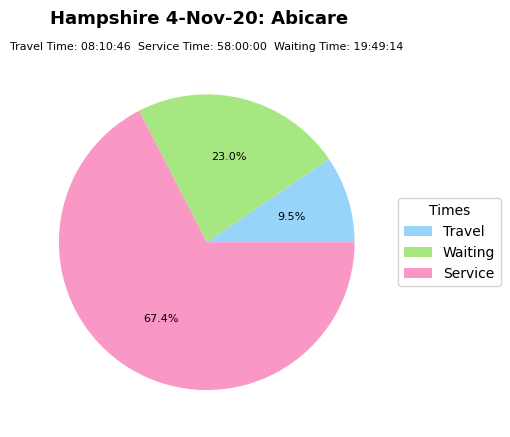
\includegraphics[width=0.5\linewidth]{figures/4_Nov_20_Hampshire_time_info_abi}%
		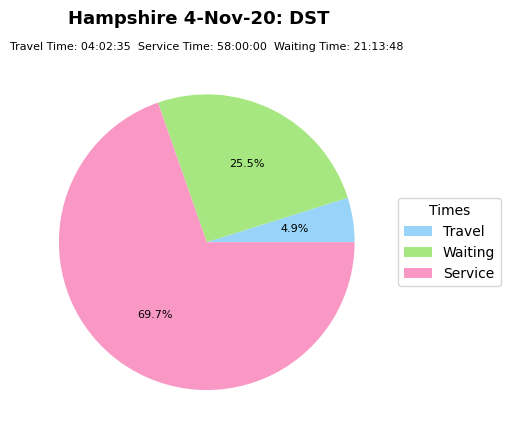
\includegraphics[width=0.5\linewidth]{figures/4_Nov_20_Hampshire_time_info_dst}
	\end{figure}
\end{frame}

\begin{frame}{Comparison}
	\begin{figure}[T]
		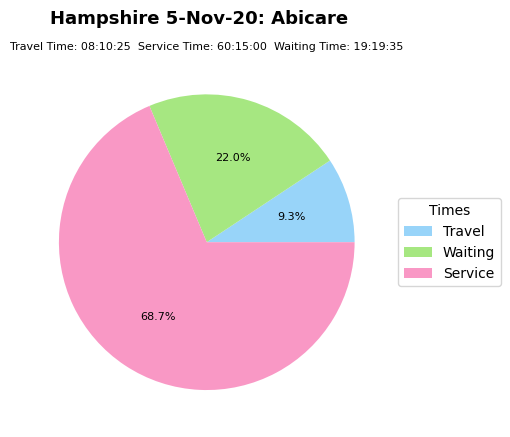
\includegraphics[width=0.5\linewidth]{figures/5_Nov_20_Hampshire_time_info_abi}%
		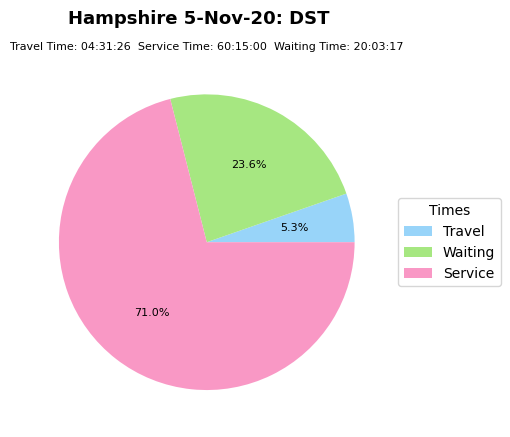
\includegraphics[width=0.5\linewidth]{figures/5_Nov_20_Hampshire_time_info_dst}
	\end{figure}
\end{frame}

\begin{frame}{Comparison}
	\begin{figure}[T]
		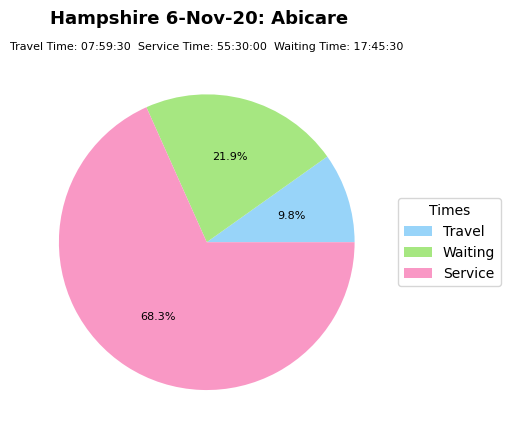
\includegraphics[width=0.5\linewidth]{figures/6_Nov_20_Hampshire_time_info_abi}%
		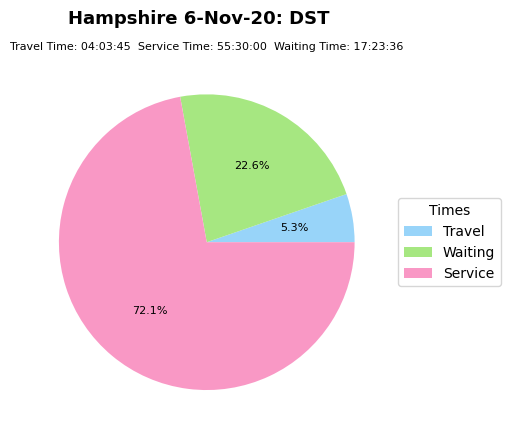
\includegraphics[width=0.5\linewidth]{figures/6_Nov_20_Hampshire_time_info_dst}
	\end{figure}
\end{frame}

\begin{frame}{Comparison}
	\begin{figure}[T]
		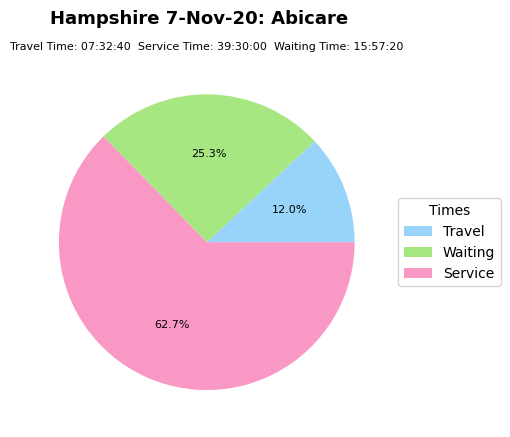
\includegraphics[width=0.5\linewidth]{figures/7_Nov_20_Hampshire_time_info_abi}%
		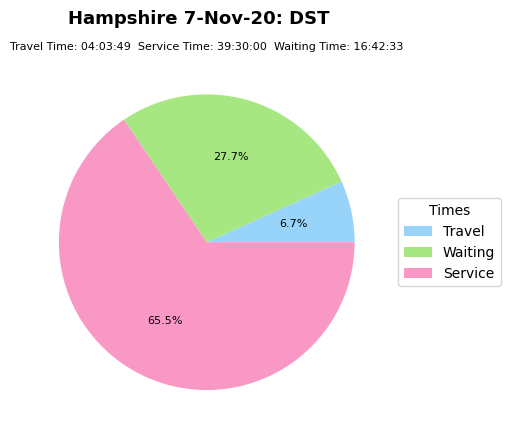
\includegraphics[width=0.5\linewidth]{figures/7_Nov_20_Hampshire_time_info_dst}
	\end{figure}
\end{frame}

\begin{frame}{Comparison}
	\begin{figure}[T]
		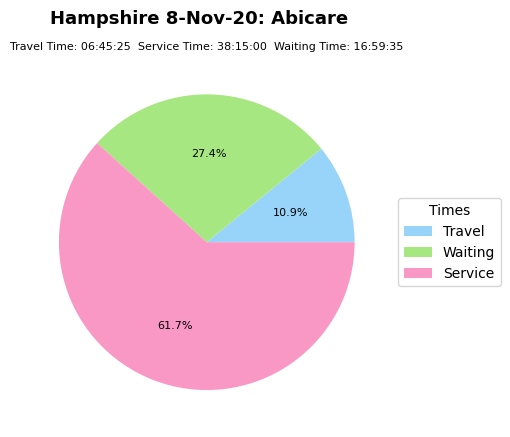
\includegraphics[width=0.5\linewidth]{figures/8_Nov_20_Hampshire_time_info_abi}%
		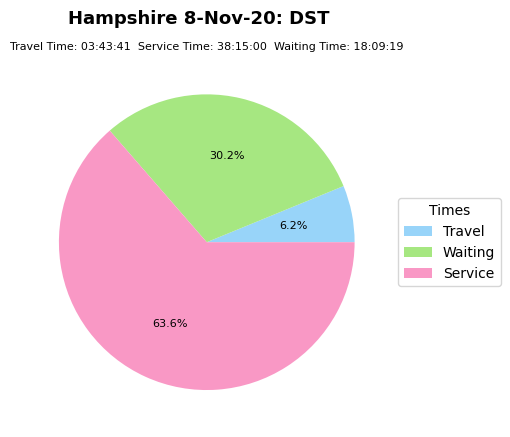
\includegraphics[width=0.5\linewidth]{figures/8_Nov_20_Hampshire_time_info_dst}
	\end{figure}
\end{frame}

\begin{frame}{Comparison}
	\begin{figure}
		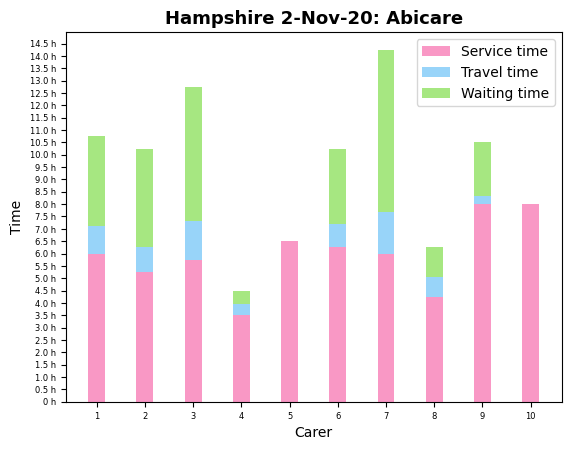
\includegraphics[width=0.5\linewidth]{figures/2_Nov_20_Hampshire_workload_abi}%
		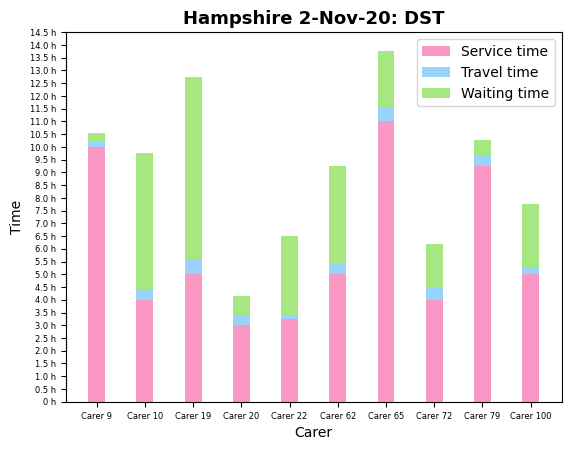
\includegraphics[width=0.5\linewidth]{figures/2_Nov_20_Hampshire_workload_dst}
	\end{figure}
\end{frame}

\begin{frame}{Comparison}
	\begin{figure}
		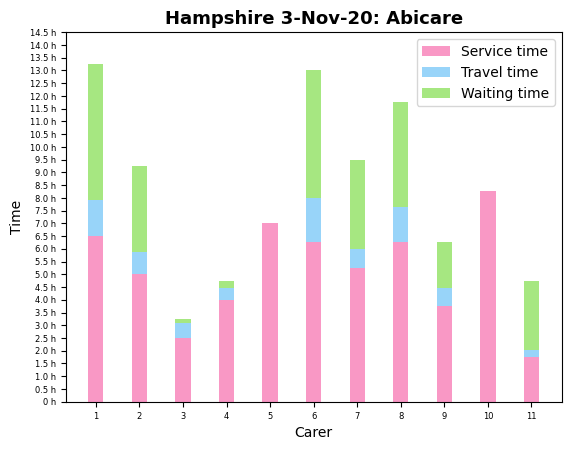
\includegraphics[width=0.5\linewidth]{figures/3_Nov_20_Hampshire_workload_abi}%
		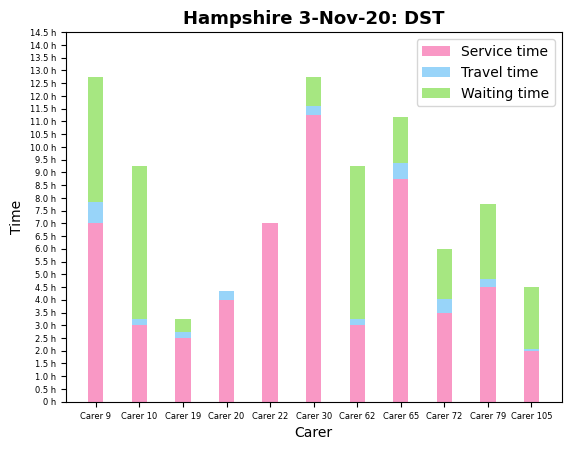
\includegraphics[width=0.5\linewidth]{figures/3_Nov_20_Hampshire_workload_dst}
	\end{figure}
\end{frame}


\begin{frame}{Comparison}
	\begin{figure}
		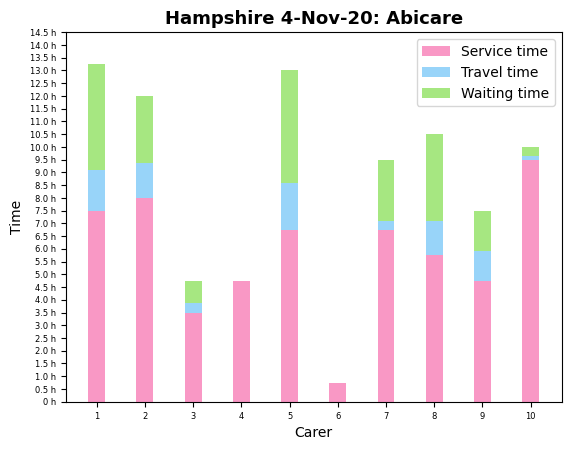
\includegraphics[width=0.5\linewidth]{figures/4_Nov_20_Hampshire_workload_abi}%
		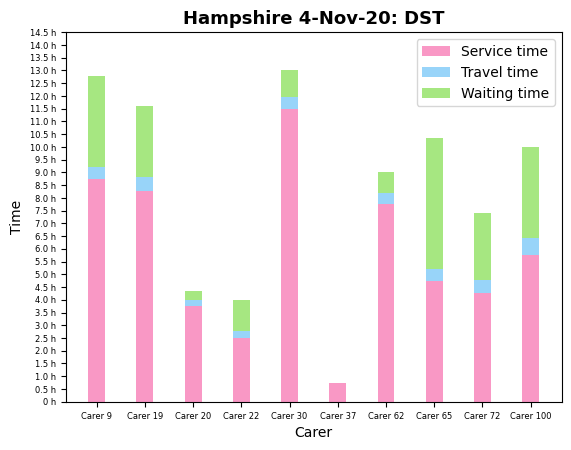
\includegraphics[width=0.5\linewidth]{figures/4_Nov_20_Hampshire_workload_dst}
	\end{figure}
\end{frame}


\begin{frame}{Comparison}
	\begin{figure}
		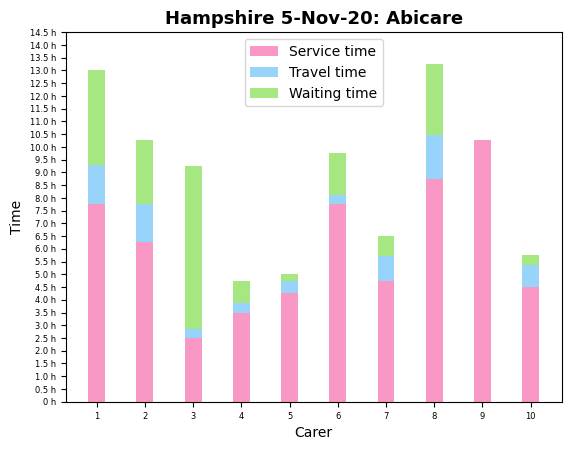
\includegraphics[width=0.5\linewidth]{figures/5_Nov_20_Hampshire_workload_abi}%
		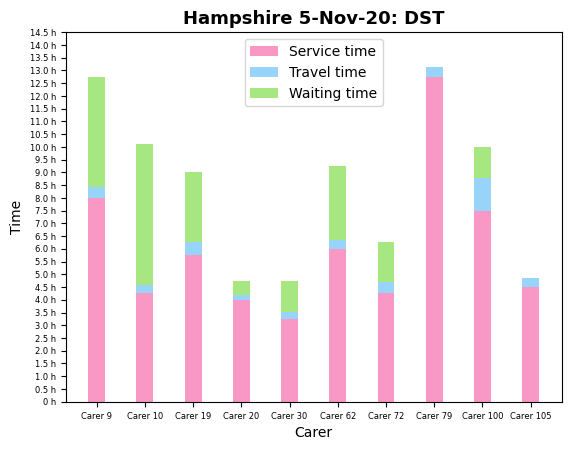
\includegraphics[width=0.5\linewidth]{figures/5_Nov_20_Hampshire_workload_dst}
	\end{figure}
\end{frame}


\begin{frame}{Comparison}
	\begin{figure}
		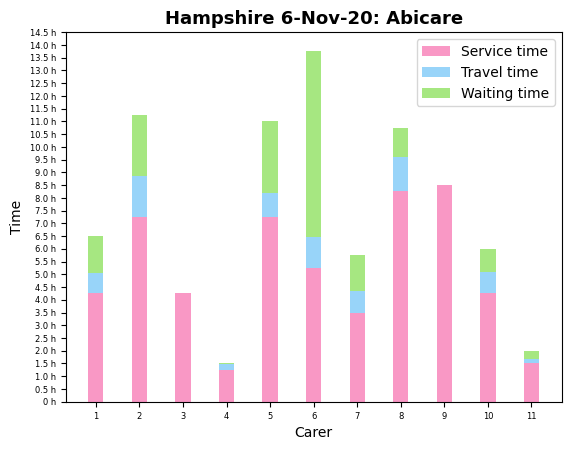
\includegraphics[width=0.5\linewidth]{figures/6_Nov_20_Hampshire_workload_abi}%
		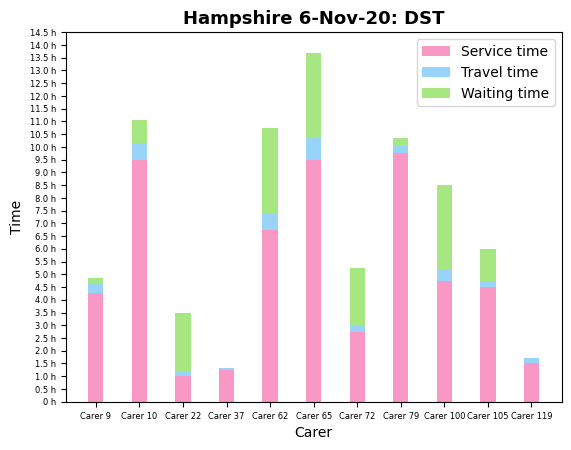
\includegraphics[width=0.5\linewidth]{figures/6_Nov_20_Hampshire_workload_dst}
	\end{figure}
\end{frame}


\begin{frame}{Comparison}
	\begin{figure}
		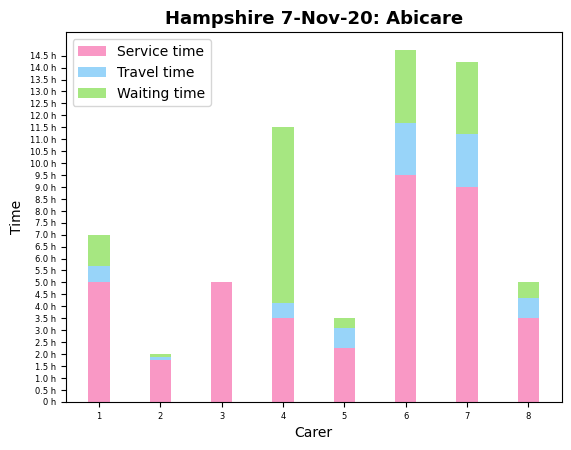
\includegraphics[width=0.5\linewidth]{figures/7_Nov_20_Hampshire_workload_abi}%
		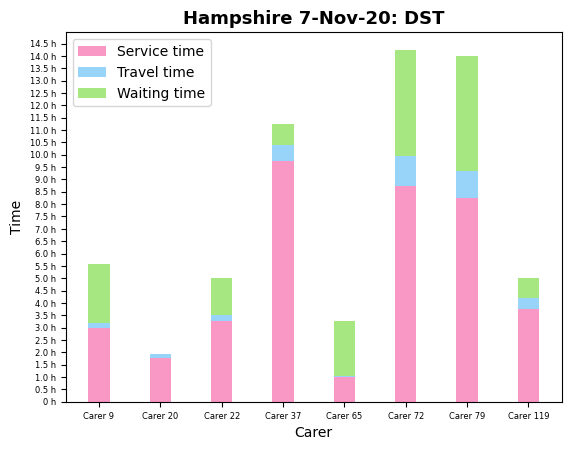
\includegraphics[width=0.5\linewidth]{figures/7_Nov_20_Hampshire_workload_dst}
	\end{figure}
\end{frame}


\begin{frame}{Comparison}
	\begin{figure}
		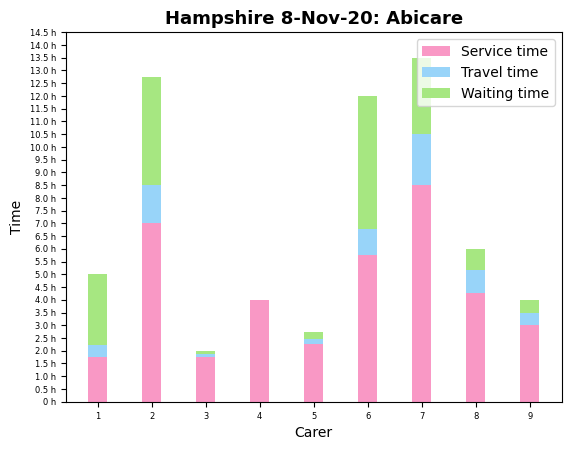
\includegraphics[width=0.5\linewidth]{figures/8_Nov_20_Hampshire_workload_abi}%
		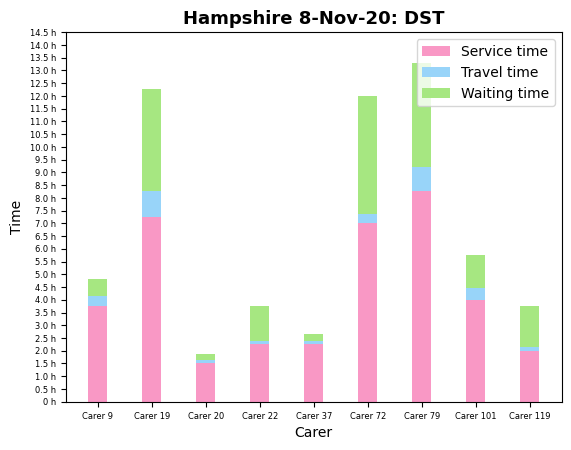
\includegraphics[width=0.5\linewidth]{figures/8_Nov_20_Hampshire_workload_dst}
	\end{figure}
\end{frame}
\end{comment}


\begin{comment}
%SAVE TEMPLATE
\begin{frame}{Comparison: Total Time (minutes)}
\scriptsize
\begin{table}
%\caption{Comparison}
\renewcommand{\arraystretch}{1.5}
\begin{tabular}{ccrrcrrcrr}\toprule
&& \multicolumn{2}{c}{Hampshire} && \multicolumn{2}{c}{Monmouth} && \multicolumn{2}{c}{Aldershot} \\
\cmidrule{3-4} \cmidrule{6-7} \cmidrule{9-10}
\multicolumn{1}{c}{Date} && \multicolumn{1}{c}{Abicare} & \multicolumn{1}{c}{DST} && \multicolumn{1}{c}{Abicare} & \multicolumn{1}{c}{DST} && \multicolumn{1}{c}{Abicare} & \multicolumn{1}{c}{DST} \\
\midrule
02-Nov && 5640.00 & 5452.46 && 6285.00 & 5851.16 && 1480.00 & 1449.90\\
03-Nov && 5460.00 & 5282.68 && 6030.00 & 5758.70 && 1080.00 & 1015.74\\
04-Nov && 5160.00 & 4996.38 && 6135.00 & 6044.82 && 1355.00 & 1321.32\\
05-Nov && 5265.00 & 5089.72 && 7200.00 & 6955.46 && 2000.00 & 1905.00\\
06-Nov && 4875.00 & 4617.36 && 7455.00 & 7100.96 && 1470.00 & 1345.28\\
07-Nov && 3780.00 & 3616.35 && 4845.00 & 4574.79 && 1065.00 & 1005.92\\
08-Nov && 3720.00 & 3608.01 && 4470.00 & 4380.78 && 1050.00 & 1006.87\\
\bottomrule
\end{tabular}
\end{table}%
\end{frame}

\begin{frame}{Comparison: Total Travel Time (minutes)}
\scriptsize
\begin{table}
%\caption{Comparison}
\renewcommand{\arraystretch}{1.5}
\begin{tabular}{ccrrcrrcrr}\toprule
&& \multicolumn{2}{c}{Hampshire} && \multicolumn{2}{c}{Monmouth} && \multicolumn{2}{c}{Aldershot} \\
\cmidrule{3-4} \cmidrule{6-7} \cmidrule{9-10}
\multicolumn{1}{c}{Date} && \multicolumn{1}{c}{Abicare} & \multicolumn{1}{c}{DST} && \multicolumn{1}{c}{Abicare} & \multicolumn{1}{c}{DST} && \multicolumn{1}{c}{Abicare} & \multicolumn{1}{c}{DST} \\
\midrule
02-Nov && 475.00 & 232.28 && 722.55 & 687.00 && 192.77 & 124.81\\
03-Nov && 489.88 & 227.02 && 728.62 & 745.88 && 166.05 & 119.21\\
04-Nov && 490.77 & 242.58 && 769.78 & 895.18 && 178.28 & 119.79\\
05-Nov && 490.42 & 271.44 && 798.20 & 687.87 && 211.58 & 122.75\\
06-Nov && 479.50 & 243.76 && 864.52 & 920.79 && 152.97 & 108.11\\
07-Nov && 452.67 & 243.81 && 694.07 & 779.27 && 167.70 & 108.08\\
08-Nov && 405.41 & 223.68 && 666.17 & 802.96 && 176.48 & 119.98\\
\bottomrule
\end{tabular}
\end{table}%
\end{frame}

\begin{frame}{Comparison: Total Waiting Time (minutes)}
	\scriptsize
	\begin{table}
		%\caption{Comparison}
		\renewcommand{\arraystretch}{1.5}
		\begin{tabular}{ccrrcrrcrr}\toprule
			&& \multicolumn{2}{c}{Hampshire} && \multicolumn{2}{c}{Monmouth} && \multicolumn{2}{c}{Aldershot} \\
			\cmidrule{3-4} \cmidrule{6-7} \cmidrule{9-10}
			\multicolumn{1}{c}{Date} && \multicolumn{1}{c}{Abicare} & \multicolumn{1}{c}{DST} && \multicolumn{1}{c}{Abicare} & \multicolumn{1}{c}{DST} && \multicolumn{1}{c}{Abicare} & \multicolumn{1}{c}{DST} \\
			\midrule
			02-Nov && 1595.00 & 1650.18 && 1407.45 & 1009.16 && 222.23 & 260.09\\
			03-Nov && 1580.12 & 1665.65 && 1026.38 & 737.81 && 73.95 & 56.53\\
			04-Nov && 1189.23 & 1273.80 && 775.22 & 559.64 && 36.72 & 61.53\\
			05-Nov && 1159.58 & 1203.28 && 1661.80 & 1527.59 && 338.42 & 332.25\\
			06-Nov && 1065.50 & 1043.60 && 1505.48 & 1095.16 && 402.03 & 322.17\\
			07-Nov && 957.33 & 1002.54 && 790.93 & 435.51 && 212.30 & 212.84\\
			08-Nov && 1019.59 & 1089.32 && 548.83 & 322.82 && 143.52 & 156.89\\
			\bottomrule
		\end{tabular}
	\end{table}%
\end{frame}
\end{comment}




\begin{comment}
\begin{frame}
\begin{figure}
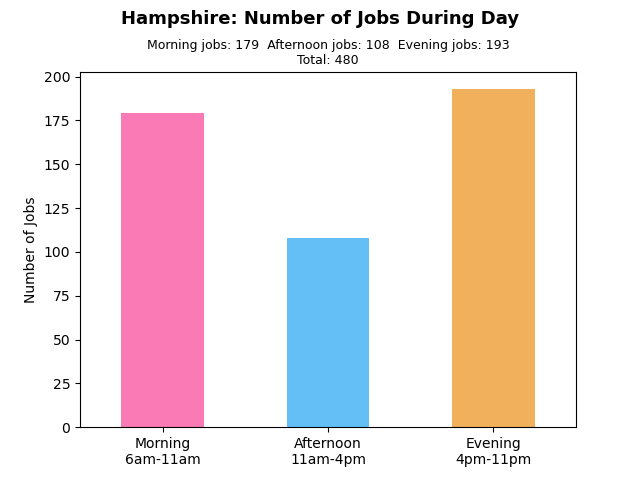
\includegraphics[width=0.5\textwidth]{figures/Hampshire_timeofday_jobs_abi}
\end{figure}
\vspace*{-0.9cm}
\begin{columns}[T]
\begin{column}{0.5\textwidth}
\begin{figure}
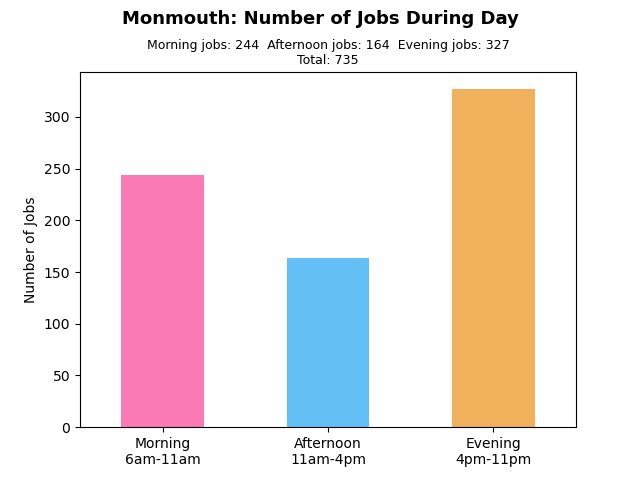
\includegraphics[width=\textwidth]{figures/Monmouth_timeofday_jobs_abi}
\end{figure}
\end{column}%
\begin{column}{0.5\textwidth}
\begin{figure}
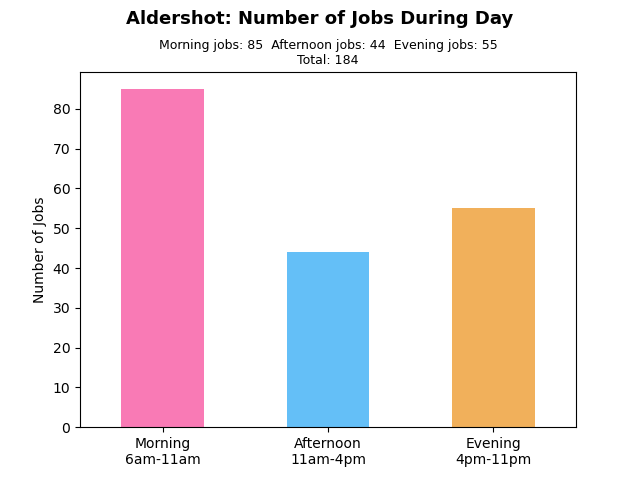
\includegraphics[width=\textwidth]{figures/Aldershot_timeofday_jobs_abi}
\end{figure}
\end{column}
\end{columns}
\end{frame}

\begin{frame}
\begin{figure}
\includegraphics[width=0.5\textwidth]{figures/Hampshire_shift_jobs_abi}
\end{figure}
\vspace*{-0.8cm}
\begin{columns}[T]
\begin{column}{0.5\textwidth}
\begin{figure}
\includegraphics[width=\textwidth]{figures/Monmouth_shift_jobs_abi}
\end{figure}
\end{column}%
\begin{column}{0.5\textwidth}
\begin{figure}
\includegraphics[width=\textwidth]{figures/Aldershot_shift_jobs_abi}
\end{figure}
\end{column}
\end{columns}
\end{frame}

\begin{frame}{Comparison}
\begin{figure}[T]
\includegraphics[width=0.5\linewidth]{figures/2_Nov_20_Hampshire_time_info_abi}%
\includegraphics[width=0.5\linewidth]{figures/2_Nov_20_Hampshire_time_info_dst}
\end{figure}
\end{frame}

\begin{frame}{Comparison}
\begin{figure}
\includegraphics[width=0.5\linewidth]{figures/2_Nov_20_Hampshire_workload_abi}%
\includegraphics[width=0.5\linewidth]{figures/2_Nov_20_Hampshire_workload_dst}
\end{figure}
\end{frame}

\begin{frame}{Comparisonx}
\begin{figure}
\includegraphics[width=0.5\linewidth]{figures/3_Nov_20_Hampshire_workload_abi}%
\includegraphics[width=0.5\linewidth]{figures/3_Nov_20_Hampshire_workload_dst}
\end{figure}
\end{frame}

\begin{frame}{Comparison}
\begin{figure}[B]
\includegraphics[width=0.5\linewidth]{figures/2_Nov_20_Monmouth_time_info_abi}%
\includegraphics[width=0.5\linewidth]{figures/2_Nov_20_Monmouth_workload_abi}
\end{figure}
\end{frame}

\begin{frame}{Comparison}
\begin{figure}
\includegraphics[width=0.5\linewidth]{figures/2_Nov_20_Aldershot_time_info_abi}%
\includegraphics[width=0.5\linewidth]{figures/2_Nov_20_Aldershot_workload_abi}
\end{figure}
\end{frame}



\begin{frame}
\begin{columns}
\column{0.5\textwidth}
\begin{minipage}[c][0.4\textheight][c]{\linewidth}
\centering
\includegraphics[width=0.9\linewidth]{figures/Hampshire_timeofday_jobs_abi}
\end{minipage}
\begin{minipage}[c][0.4\textheight][c]{\linewidth}
\centering
\includegraphics[width=0.9\linewidth]{figures/Monmouth_timeofday_jobs_abi}
\end{minipage}
\column{0.5\textwidth}
\begin{minipage}[c][0.4\textheight][c]{\linewidth}
\begin{enumerate}
\item First.
\item Second.
\item Third.
\end{enumerate}
\end{minipage}
\begin{minipage}[c][0.4\textheight][c]{\linewidth}
\centering
\includegraphics[width=0.9\linewidth]{figures/Aldershot_timeofday_jobs_abi}
\end{minipage}
\end{columns}
\end{frame}


\begin{frame}
\scriptsize
\begin{multicols}{3}
\begin{table}
\setlength{\tabcolsep}{3pt}
\renewcommand{\arraystretch}{1.5}
%		\caption{Hampshire}
\begin{tabular}{ccc}\toprule
Date & Abicare & DST \\
\midrule
02-Nov & 5640.00 & 5452.46\\
03-Nov & 5460.00 & 5282.68\\
04-Nov & 5160.00 & 4996.38\\
05-Nov & 5265.00 & 5089.72\\
06-Nov & 4875.00 & 4617.36 \\
07-Nov & 3780.00 & 3616.35\\
08-Nov & 3720.00 & 3608.01\\
\bottomrule
\end{tabular}
\end{table}%
\vspace{2mm}
\begin{table}
\setlength{\tabcolsep}{3pt}
\renewcommand{\arraystretch}{1.5}
\begin{tabular}{ccc}\toprule
Date & Abicare & DST \\
\midrule
02-Nov & 6285.00 & 5851.16\\
03-Nov & 6030.00 & 5758.70\\
04-Nov & 6135.00 & 6044.82\\
05-Nov & 7200.00 & 6955.46\\
06-Nov & 7455.00 & 7100.96 \\
07-Nov & 4845.00 & 4574.79\\
08-Nov & 4470.00 & 4380.78\\
\bottomrule
\end{tabular}
\end{table}%
\vspace{2mm}
\begin{table}
\setlength{\tabcolsep}{3pt}
\renewcommand{\arraystretch}{1.5}
\begin{tabular}{ccc}\toprule
Date & Abicare & DST \\
\midrule
02-Nov & 1480.00 & 1449.90\\
03-Nov & 1080.00 & 1015.74\\
04-Nov & 1355.00 & 1321.32\\
05-Nov & 2000.00 & 1905.00\\
06-Nov & 1470.00 & 1345.28 \\
07-Nov & 1065.00 & 1005.92\\
08-Nov & 1050.00 & 1006.87\\
\bottomrule
\end{tabular}
\end{table}
\end{multicols}
\end{frame}
\end{comment}


\end{document}